\documentclass{beamer}

% \usepackage{biblatex}
% \addbibresource{references.bib}

\usepackage[small,nohug,heads=vee]{diagrams}
\diagramstyle[labelstyle=\scriptstyle]
\usepackage{caption}
\usepackage{subcaption}
\usepackage{mathtools}
\usepackage{listings}
\lstset{
  columns=flexible,
  mathescape=true,
  keepspaces=true,
  showstringspaces=false,
  stringstyle=\slshape\color{green!40!black},
  basicstyle=\ttfamily\small,
  language=SQL,
  morekeywords={*, self},
  commentstyle=\slshape\color{black!60},
  tabsize=2,
}

\newcommand{\B}{\mathbb B} % complex numbers
\newcommand{\C}{\mathbb C} % complex numbers
\newcommand{\N}{\mathbb N} % the natural numbers
\newcommand{\R}{\mathbb R} % the real numbers
\newcommand{\Q}{\mathbb Q} % the rational numbers
\newcommand{\D}{\mathbf D} % bold-face D, used for generic domain
\newcommand{\SR}{\mathbf S} % semiring
\newcommand{\dleq}{\mbox{ :- }}
\newcommand{\deq}{\stackrel{\text{def}}{=}}

\newcommand{\set}[1]{\{#1\}}                    % Set (as in \set{1,2,3}).
\newcommand{\setof}[2]{\{{#1}\mid{#2}\}}        % Set (as in \setof{x}{x>0}).

\usetheme{metropolis}           % Use metropolis theme
% \setbeameroption{show only notes}
\setbeameroption{hide notes}

\title{Optimizing Modern Data Processing Systems with Automated Reasoning}
\date{\today}
\author{Remy Wang}
\institute{University of Washington}
\begin{document}
  \maketitle
  \note{yo}

  \begin{frame}{Overview}
    \note{sup}
    \tableofcontents
  \end{frame}

  \section{Modern Data Processing}

  \begin{frame}{Modern Data Processing: Queries}
    \note{blah}
    Betweenness centrality of a graph $E$:
    \begin{align*}
      C(s, v) = \sum_{t: E(v, t) \wedge D(s, t)=D(s, v+1)} 
      \frac{\sigma(s, v)}{\sigma(s, t)}(1+ C(s, t))
    \end{align*}
    where $D$ is the distance, $\sigma$ is the \# of shortest paths. \pause
    \begin{itemize}
      \item Non-relational data \pause
      \item Aggregation \& interpreted functions \pause
      \item Recursive \pause
     \end{itemize}
    \textbf{Expressiveness} not well-supported by traditional optimizers:
    \[\#[R \times S] \Rightarrow \#[R] \cdot \#[S]\]
  \end{frame}

  \begin{frame}{Modern Data Processing: Data}
    \begin{columns}
      \begin{column}{{0.5\textwidth}}
        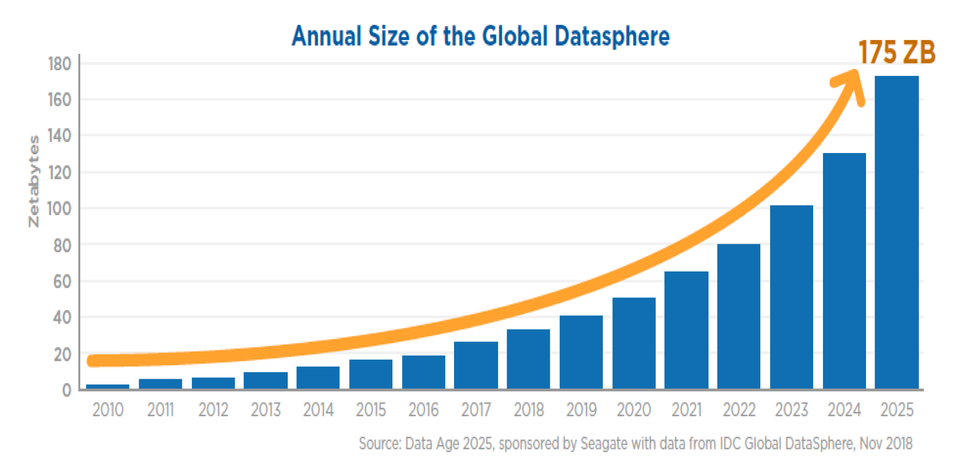
\includegraphics[width=\linewidth]{datasphere.png}
      \end{column}
      \begin{column}{{0.5\textwidth}}
        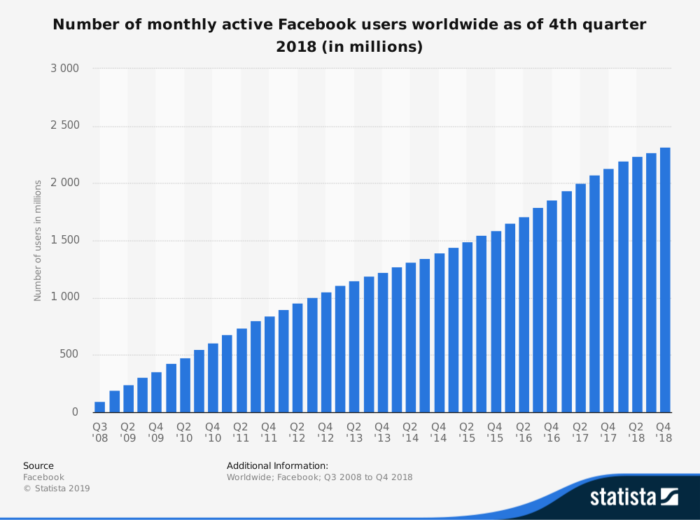
\includegraphics[width=\linewidth]{fb.png}
      \end{column}
    \end{columns}
    \begin{itemize}
      \item Data is increasing in \textbf{volume} \& \textbf{velocity} \pause
      \item The optimizer needs to produce faster plans in shorter time
    \end{itemize}
  \end{frame}

  \begin{frame}{Modern Data Processing: Systems}
    \begin{figure}
    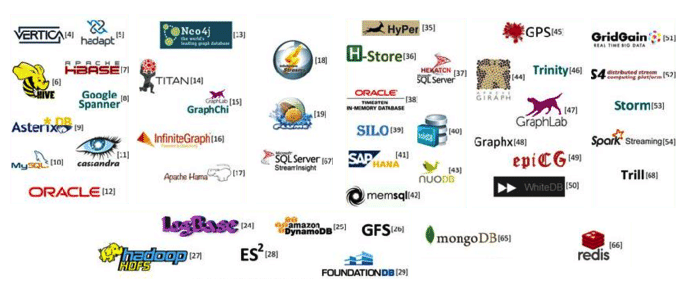
\includegraphics[width=\linewidth]{systems.png}
    \end{figure}
    \begin{itemize}
      \item Every data processing system needs an optimizer!
      \item Simplifying optimizers can save a lot of time for everyone.
    \end{itemize}
  \end{frame}

  \begin{frame}{My Theses}
    \begin{itemize}
      \item Core components and techniques from \textbf{automated reasoning}
      can make query optimizers simpler, more efficient,
      and more effective. \pause
      \item The \textbf{functional representation} of data can enable query 
      optimizers to effectively leverage automated reasoning tools.
    \end{itemize}
  \end{frame}

  \section{Background: Query Optimization and Reasoning}
  \begin{frame}{Query Optimization}
    \begin{figure}
      \includegraphics[width=0.7\linewidth]{opt.pdf}
    \end{figure}
    Given an input query and constraints on the data, 
    output an equivalent query that is more efficient. \pause \\
    This is a \textbf{synthesis problem}: given a specification,
    output a program that satisfies the spec.
  \end{frame}

  \begin{frame}{Query Optimization}
    A related problem: given constraints ($\Sigma$) on the data ($I$), 
    check if two queries ($\psi, \phi$) are equivalent.
    \[\forall I . \Sigma(I) \implies (\psi(I) = \phi(I)) \] \pause
    This is a \textbf{verification problem}:
    given a specification, check that a program meets the specification.
  \end{frame}

  \begin{frame}{Automated Reasoning}
    Both verification problems and synthesis problems are studied 
    extensively in automated reasoning.
  \end{frame}

  \begin{frame}{Automated Reasoning for Data Processing}
    \textbf{The Chase} is an algorithm that has wide applications 
    in data management. It has the property:
    \begin{alertblock}{The Chase preserves query equivalence}
      Chasing a query $Q$ with a set of integrity constraints $\Sigma$
      results in a query $Q'$ s.t.~$\Sigma \models Q'\equiv Q$.
    \end{alertblock}
  \end{frame}

  \begin{frame}{Automated Reasoning for Data Processing}
    \textbf{Chase \& Backchase}~\cite{backchase}: Given $Q$, find the smallest~\footnote{
      Refer to~\cite{backchase} for a formal definition of ``small''.
    }
    query $Q'$ s.t.~$Q'\equiv Q$.
    \begin{figure}
      \includegraphics[width=0.3\linewidth]{backchase.pdf}
    \end{figure}
    First chase the input into a {\em universal} plan $\hat Q$, \pause 
    then check if any subplan $Q'$ of $\hat Q$ is equiv.~to $Q$,
    by chasing $Q'$.
  \end{frame}

  \begin{frame}{Automated Reasoning for Data Processing}
    \textbf{Tree Automata} can capture certain class of
    relational queries, by coding tree-like data with trees.
    \begin{figure}
      \colorbox{white}{
      \includegraphics[width=0.3\linewidth]{tree1.pdf}
      \hspace{1cm}
      \includegraphics[width=0.3\linewidth]{tree2.pdf}}
    \end{figure}
    \pause
    Emptiness of tree automata is \textbf{decidable}! \\
    Check query containment: 
    $Q_1 \subseteq Q_2 \rightarrow A_{Q_1 \wedge \neg Q_2} = \emptyset$
  \end{frame}

  \begin{frame}{Automated Reasoning for Data Processing}
    \textbf{Axiomatic Rewriting} proves equivalence by chaining together 
    a sequence of axioms. \pause
    Rule-based query optimizers essentially implement that, for example:
    \[\forall R, S, p: \sigma_p (R\bowtie S) \equiv \sigma_p(R) \bowtie \sigma_p(S)\]
    corresponds to the ``push-down selection'' rewrite.\pause

    If two queries can rewrite to each other, they are equivalent.
  \end{frame}

  \begin{frame}{Automated Reasoning for Data Processing}
    \textbf{Program Verification} checks if a program satisfies a specification:
    \[\Psi(Q_{\text{in}}, Q) \stackrel{def}{=} \forall \bar R : Q_{\text{in}}(\bar R) = Q(\bar R)\]
    which is valid if $Q_{\text{in}}(\bar R) \neq Q(\bar R)$ is UNSAT (no model for $\bar R$). \pause

    \textbf{Program Synthesis} generates a program satisfying a specification:
    \[\Phi(Q_{\text{in}}) \stackrel{def}{=} \forall \bar R : Q_{\text{in}}(\bar R) = Q(\bar R)\]
    which gives a solution when there is a model for $Q$.
  \end{frame}

  \begin{frame}{Mismatch of Reasoning and Modern Data Processing}
    \begin{itemize}
      \item Logic assume set semantics; but data processing needs bag/beyond-bag semantics. \pause
      \item Logics w/ aggregates exist, but no support in well-engineered reasoners (SMT solvers). \pause
      \item Most system developers don't have deep knowledge on logic. 
    \end{itemize}    
  \end{frame}

  \begin{frame}{Mismatch of Reasoning and Modern Data Processing}
    \textbf{Need:} simple ways to reason about the expressive semantics and operations in modern 
    data processing. \pause

    \textbf{Solution:} functional representation + axiomatic rewrite + SMT
  \end{frame}
  
  \section{Functional Representation of Data}
  \begin{frame}{The Functional Representation of Data}
    Generalize every relation $R : \D^a$ to a function 
    $f_R : \D^a \rightarrow \SR$,
    where $\SR$ is a commutative semiring~\cite{semiring}. \pause
    \begin{itemize}
      \item A $\B$-relation is a standard relation under \textbf{set} semantics. \pause
      \item An $\N$-relation is a standard relation under \textbf{bag} semantics. \pause
      \item When $\D = [n]$, an $\R$-relation is a tensor over the reals.
    \end{itemize}
  \end{frame}

  \begin{frame}{The Functional Representation of Data}
    An expression in $\SR$-relational algebra is one of:
    \begin{enumerate}
      \item An \textbf{atom} $r$ of the form $R(x_1, ..., x_a)$.
      \item A \textbf{natural join} of two expressions $e_1 \times e_2$.
      \item A \textbf{union} of two expressions, $e_1 + e_2$.
      \item An \textbf{aggregate},  $\sum_x e$.
    \end{enumerate} \pause
    A variable $x$ is \textbf{bound} in $e$ if $e$ contains $\sum_x e'$;
    otherwise it is \textbf{free}. \pause 
    Every atom $R(x_1, ..., x_a)$ evaluates to some $s \in \SR$, and
    $+, \times$ and $\sum$ compute over $\SR$.
  \end{frame}

  \begin{frame}{The Functional Representation of Data}
    $\sum_y E(x, y) \times E(y, z)$ specializes to 
    different semantics under different semiring $\SR$:
    \begin{enumerate}
      \item Under $(\mathbb{B},\vee, \wedge, \texttt{false}, \texttt{true})$
          it is the binary join $Q(x, z) \dleq \exists y: E(x, y) \wedge E(y, z).$ 
          under set semantics. \pause
      \item Under $(\mathbb{N}, +, \times, 0, 1)$ it is under
          bag semantics. \pause
      \item Under $(\mathbb{R}, +, \times, 0, 1)$ it computes the matrix product $EE$. \pause
      \item Under $(\mathbb{N} \cup \set{\infty}, \min, +, \infty, 0)$ it computes the lengths
          of all shortest 2-paths in a graph:
          $Q(x, z) = \min_y E(x, y) + E(y, z)$
  \end{enumerate}
  \end{frame}

  \begin{frame}{The Functional Representation of Data}
    \textbf{Query Equivalence} Two queries
    $Q_1({\bar R})$, $Q_2({\bar R})$
    over $\SR$-relations ${\bar R}$ with domain $\mathbf{D}$
    are equivalent iff
    they denote the same function:
    \begin{align*}
    Q_1 =_{\SR,\D} Q_2 \iff
    \forall {\bar x}:\D^a, {\bar R} :
    Q_1({\bar R})({\bar x}) =_{\SR}
    Q_2({\bar R})({\bar x})
    \end{align*} \pause
    Write $=_{\SR}$ for equiv.~over all domains;
    $=$ for equiv.~over all domains and codomains.
  \end{frame}

  \begin{frame}{The Functional Representation of Data}
    \alert{Isomorphism Captures Equivalence} ($\bigstar$)~\cite{spores}
    Let $e_1, e_2$ be two  canonical expressions.
    Then the following conditions are equivalent:
    \begin{itemize}
  % \itemsep0em
    \item \label{item:1} $e_1 \equiv e_2$ (they are isomorphic)
    \item \label{item:2} $e_1 = e_2$ (they are equivalent over all semirings)
    \item \label{item:3} $e_1 =_\C e_2$, $e_1 =_\R e_2$, and $e_1 =_\N e_2$
    \item \label{item:6} $e_1 =_{\N, \D} e_2$ for finite $\D$
    s.t. $|\D| \geq \max(|vars(e_1)|, |vars(e_2)|)$.
    \end{itemize} \pause
    We can change equivalence after changing $\SR$ to $\N$, $\R$, or $\C$ (SMT),
    or by canonizing \& checking isomorphism (axiomatic rewrite).
  \end{frame}

  \begin{frame}{The Functional Representation of Data}
    \textbf{Summary} The functional representation of data enables us to:
    \begin{enumerate}
      \item Capture the diverse semantics in modern analytics.
      \item Reason about queries using well-established techniques.
    \end{enumerate}
  \end{frame}
  
  \section{Building Optimizers that Reason}

  \begin{frame}{Building Optimizers that Reason}
    \onslide<1-2>{\textbf{Program Verification} checks if a program satisfies a specification:
    \[\Psi(Q_{\text{in}}, Q) \stackrel{def}{=} \forall \bar R : Q_{\text{in}}(\bar R) = Q(\bar R)\]
    which is valid if $Q_{\text{in}}(\bar R) \neq Q(\bar R)$ is UNSAT (no model for $\bar R$).}

    \onslide<1>{\textbf{Program Synthesis} generates a program satisfying a specification:
    \[\Phi(Q_{\text{in}}) \stackrel{def}{=} \forall \bar R : Q_{\text{in}}(\bar R) = Q(\bar R)\]
    which gives a solution when there is a model for $Q$.}
  \end{frame}

  \begin{frame}{Verifying Equivalence}
    \textbf{Challenges}
    \begin{itemize}
      \item Not all domain types are well-supported ($\N \cup \set{\infty}$, $\R$).
      \item Hard to encode $\sum$; unfolding is unsound \& blows up
    \end{itemize}
  \end{frame}
  
  \begin{frame}{Verifying Equivalence}
    \textbf{Solution} To support domain types: Theorem ($\bigstar$) 
    allows us to switch to the $\N$-semiring to check equivalence. \pause
    
    To verify the commutativity of join, solve for: 
    \[f_R(x, y) \times f_S(y, z) \neq f_S(y, z) \times f_R(x, y)\]
    where $x, y, z$ are natural numbers, $f_R, f_S$ are uninterpreted
    functions of type $\N \times \N \rightarrow \N$. 
  \end{frame}

  \begin{frame}{Verifying Equivalence}
    \textbf{Solution} To encode $\sum$: Introduce an uninterpreted function
    \[f_{\Sigma}:\N\times \N \rightarrow \N\] 
    and encode every aggregation $\sum_x e$ with $f_{\Sigma}(x, e)$. \pause

    \textbf{Soundness}: $f_{\Sigma}(x_1, e_1) \neq f_{\Sigma}(x_2, e_2)$ only
    if $x_1 \neq x_2$ or $e_1 \neq e_2$.\pause

    \textbf{Incompleteness}: cannot prove 
    e.g.~$\sum_x e_1 + \sum_x e_2 = \sum_x e_1 + e_2$.
  \end{frame}

  \begin{frame}{Verifying Equivalence}
    \textbf{Solution} Alternatively, canonize \& check for isomorphism:
    \[Q_1 \xrightarrow[]{\text{canonize}} \equiv \xleftarrow[]{\text{canonize}} Q_2\]
    Complete by ($\bigstar$) for {\em pure} $\SR$-RA expressions; \pause
    augment with SMT to reason about interpreted functions:
    \[Q_1 \xrightarrow[]{\text{canonize}} \text{SMT} \xleftarrow[]{\text{canonize}} Q_2\]
  \end{frame}

  \begin{frame}{Exploring Query Plans}
    \begin{figure}
      \includegraphics[width=0.7\linewidth]{opt.pdf}
    \end{figure}
    2 ways to explore search equivalence space / search efficient space
  \end{frame}

  \begin{frame}{Searching the Equivalence Space}
    Grow a collection of equivalence plans \& find the cheapest. \pause

    An \textbf{E-Graph}~\cite{eqsat} is a compact data structure to store collections 
    of equivalent expressions:
    \begin{figure}
      \includegraphics[width=0.3\linewidth]{fgn.pdf}
    \end{figure}
    Group \& share equiv.~subexpressions: there are $\Omega(N^2)$ expr.~above!
  \end{frame}

  \begin{frame}{Searching the Equivalence Space}
    Grow an e-graph by applying rewrite rules:
    \begin{figure}
      \includegraphics[width=0.3\linewidth]{fgn.pdf}
    \end{figure}
    while preserving \textbf{congruence}: 
    \[\forall f : \bigwedge_{i \in [k]} x_i \equiv y_i \implies f(x_1, \ldots, x_k ) \equiv f(y_1, \ldots, y_k)\]
  \end{frame}

  \begin{frame}{Searching the Equivalence Space}
    Generate a boolean variable per operation ($B_{op}$) and 
    one per equivalence class ($B_{c}$), then solve~\cite{eqsat} :
    \begin{align*}
      Constraints &\deq B_r \wedge \bigwedge_{op} F(op) \wedge \bigwedge_c G(c)
      \\ F(op) &\deq B_{op} \rightarrow \bigwedge_{c \in op.children} B_c \\ G(c)
      &\deq B_c \rightarrow \bigvee_{op \in c.nodes} B_{op}
      \end{align*}
      \[\textbf{minimize} \sum_{op} B_{op} \cdot C_{op} \textbf{ s.t. } Constraints\]
  \end{frame}

  \begin{frame}{Searching the Efficient Space}
    \begin{figure}
      \includegraphics[width=0.7\linewidth]{opt.pdf}
    \end{figure}
    Search among the efficient plans for one equivalent to the input.
  \end{frame}

  \begin{frame}{Searching the Efficient Space}
    \textbf{Goal} To optimize an expensive recursive query:
    \[Q \deq G(F(\cdots F(\bar R))) \text{ (apply $F$ to a fixpoint)}\] \pause
    \textbf{Solution}~\cite{dove} Find a function $H$ such that:
    \[\forall \bar R : H^*(G(\bar R)) = G(F^*(\bar R))\]
    More efficient when $G$ reduces dimension!
  \end{frame}

  \begin{frame}{Searching the Efficient Space}
    Sufficient to find $H$ s.t.~$H\circ G \equiv G \circ F$:
    \begin{diagram}
      X_0   & \rTo^F & X_1 & \rTo^F & X_2 & \ldots & \rTo^F & X_n\\
     \dTo^G  &            & \dTo^G    &            & \dTo^G    &        &            & \dTo^G\\
      Y_0        & \rTo^H & Y_1 & \rTo^H & Y_2 & \ldots & \rTo^H & Y_n
  \end{diagram}  
  \end{frame}

  \begin{frame}{Searching the Efficient Space}
    How to find $H$? ``Generate \& check'':
    \begin{figure}
      \includegraphics[width=0.7\linewidth]{cegis.pdf}
    \end{figure}
    Enumerate all $\SR$-RA expressions until 
    finding $H$ s.t.~$H\circ G \equiv G \circ F$ \pause

    Hopelessly inefficient!
  \end{frame}

  \begin{frame}{Searching the Efficient Space}
    How to find $H$? Counterexample-guided Synthesis (CEGIS)~\cite{sketch}:
    \begin{figure}
      \includegraphics[width=0.7\linewidth]{cegis.pdf}
    \end{figure}
    Implement both the generator \& checker with an SMT solver \\
    Guide generation of plans by {\em counterexamples} from the checker
  \end{frame}

  \begin{frame}{Searching the Efficient Space}
    \textbf{Challenge} CEGIS requires the checker \& the generator to 
    be implemented entirely in SMT. \pause \\
    But we'd like to combine SMT with rewriting:
    \[Q_1 \xrightarrow[]{\text{canonize}} \text{SMT} \xleftarrow[]{\text{canonize}} Q_2\]\pause
    \textbf{Solution}~\cite{dove} Canonize input query $G \circ F$ before CEGIS,
    then constrain grammar to only generate {\em canonical} plans that 
    can be ``denormalized'' into $H\circ G$.
    \[Q_1 \xrightarrow[]{\text{canonize}} \text{CEGIS} \xrightarrow[]{\text{denormalize}} Q_2\]
  \end{frame}

  \begin{frame}{Building Optimizers that Reason}
    \textbf{Summary}
    \begin{itemize}
      \item Automated reasoning can verify query equivalence.
      \item Both SMT solvers and rewriting can reason about queries.
      \item We can explore the search space with reasoning.
    \end{itemize}
  \end{frame}

  \begin{frame}{Result: Optimizing Linear Algebra}
    VLDB'20~\cite{spores}
    \begin{figure}
        \includegraphics[width=0.6\textwidth]{runtime.pdf}
        \caption*{My optimizer (SPORES) against SystemML}
    \end{figure}
  \end{frame}

  \begin{frame}{Result: Optimizing Linear Algebra}
    VLDB'20~\cite{spores}
    \begin{figure}
      \includegraphics[width=0.7\textwidth]{tf.pdf}
      \caption*{My optimizer (SPORES) against TensorFlow}
    \end{figure}
  \end{frame}

  \begin{frame}{Result: Optimizing Deep Learning Inference}
    MLSys'21~\cite{tensat}
    \begin{figure}
      \includegraphics[width=0.6\textwidth]{all_speedup.pdf}
      \caption*{My optimizer (Tensat) against TASO, inference speedup}
    \end{figure}
  \end{frame}

  \begin{frame}{Result: Optimizing Deep Learning Inference}
    MLSys'21~\cite{tensat}
    \begin{figure}
      \includegraphics[width=0.6\textwidth]{all_optim_time.pdf}
      \caption*{My optimizer (Tensat) against TASO, compile time}
    \end{figure}
  \end{frame}
  
  \begin{frame}{Result: Optimizing Recursion}
    SIGMOD'22 (Conditional Accept)
    \begin{figure}
      \begin{subfigure}[b]{0.4\textwidth}
        \centering
        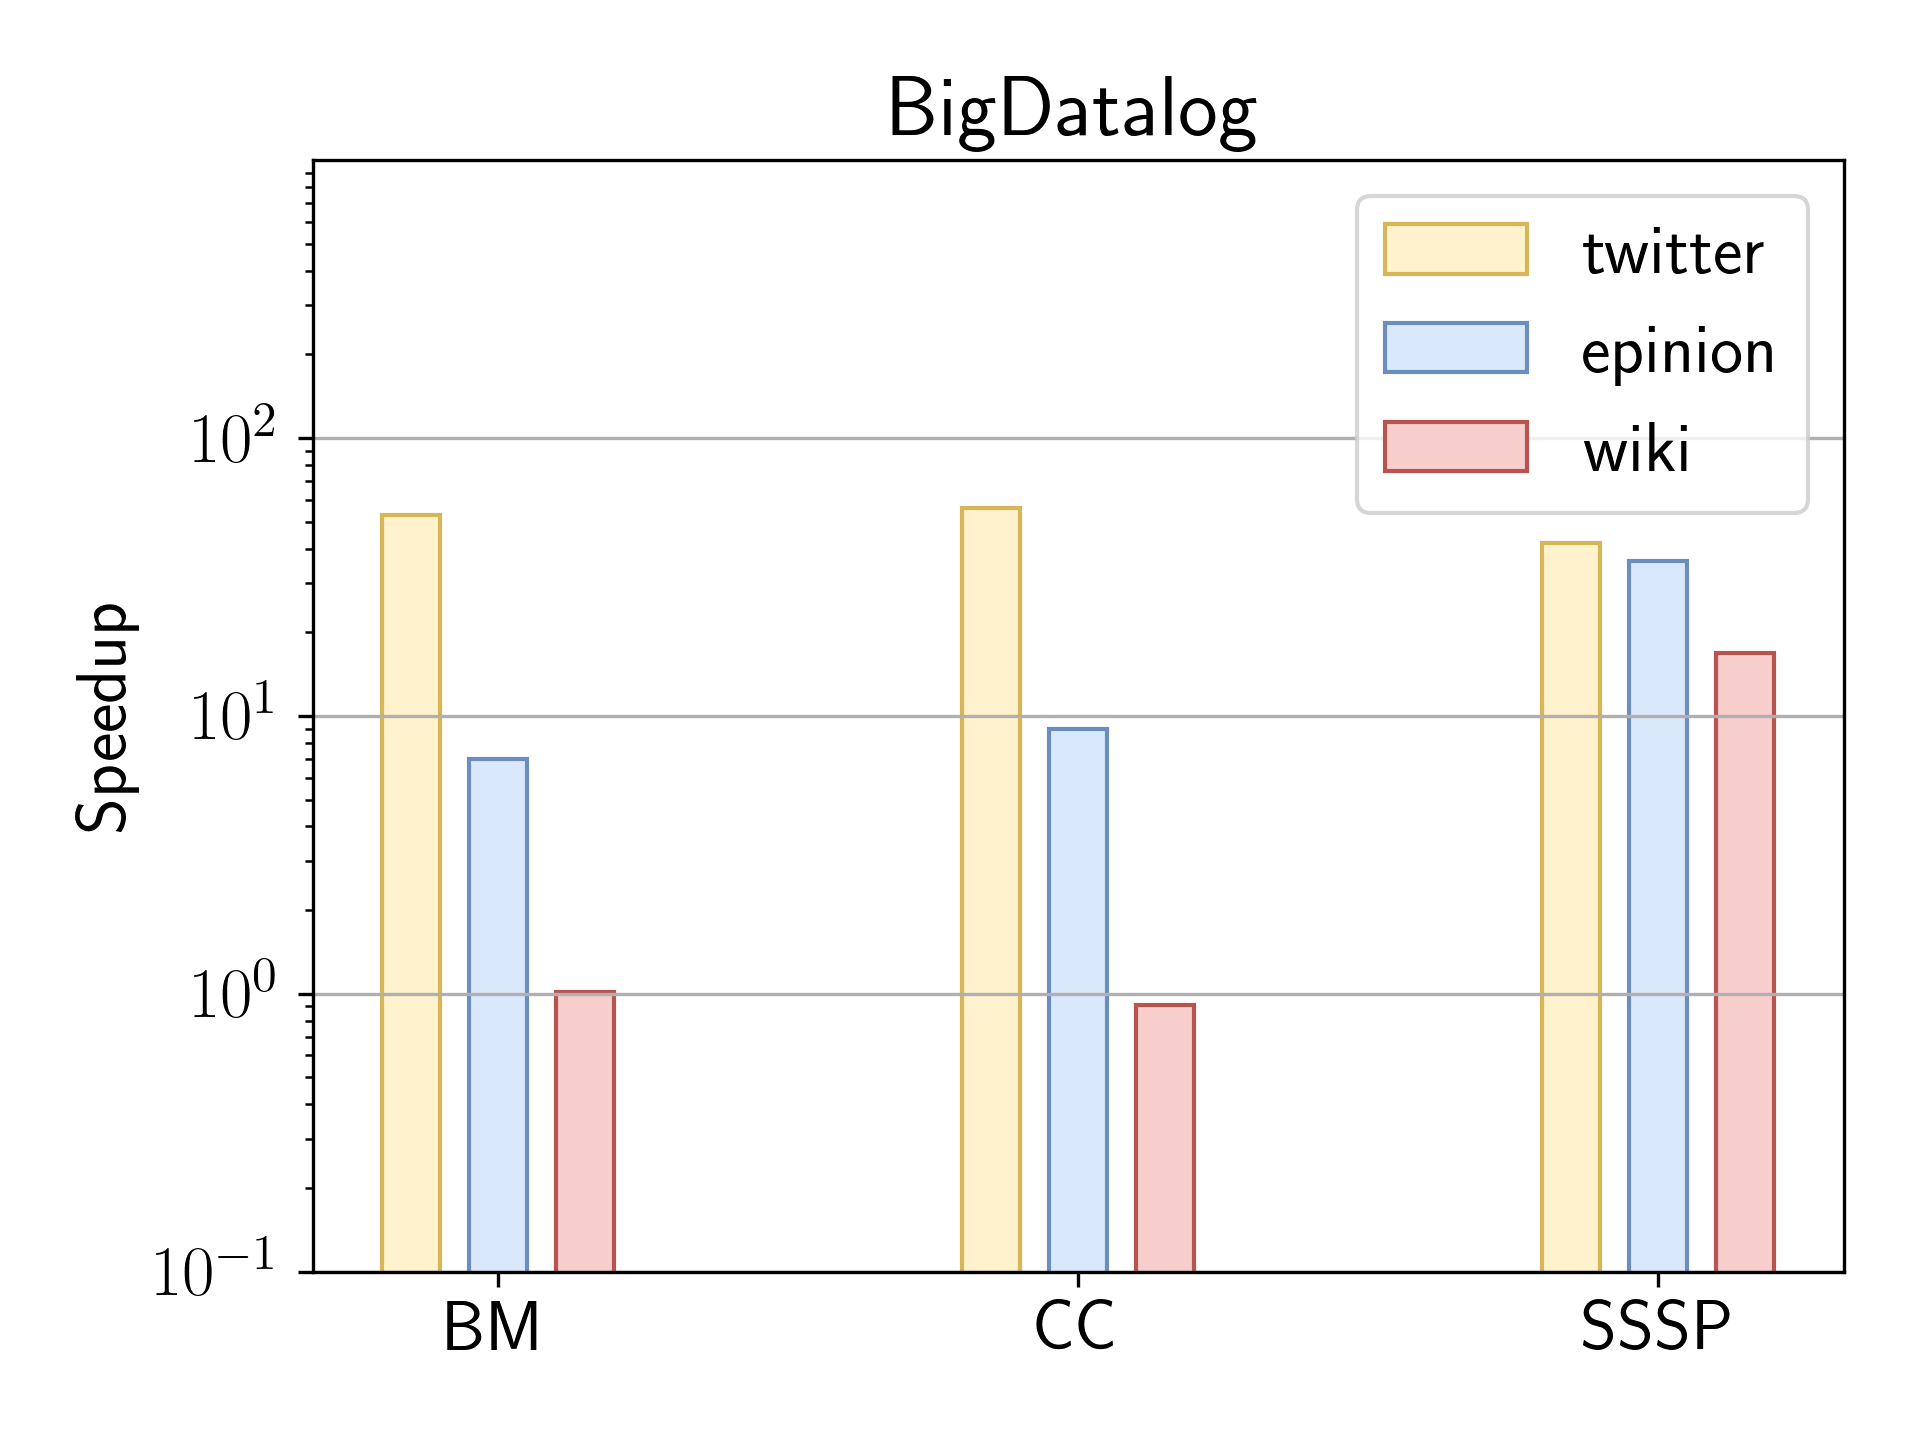
\includegraphics[width=\textwidth]{basic-bd}
        % \caption{BigDatalog}\label{fig:eval:basic:bd}
      \end{subfigure}
      \hfill
      \begin{subfigure}[b]{0.4\textwidth}
        \centering
        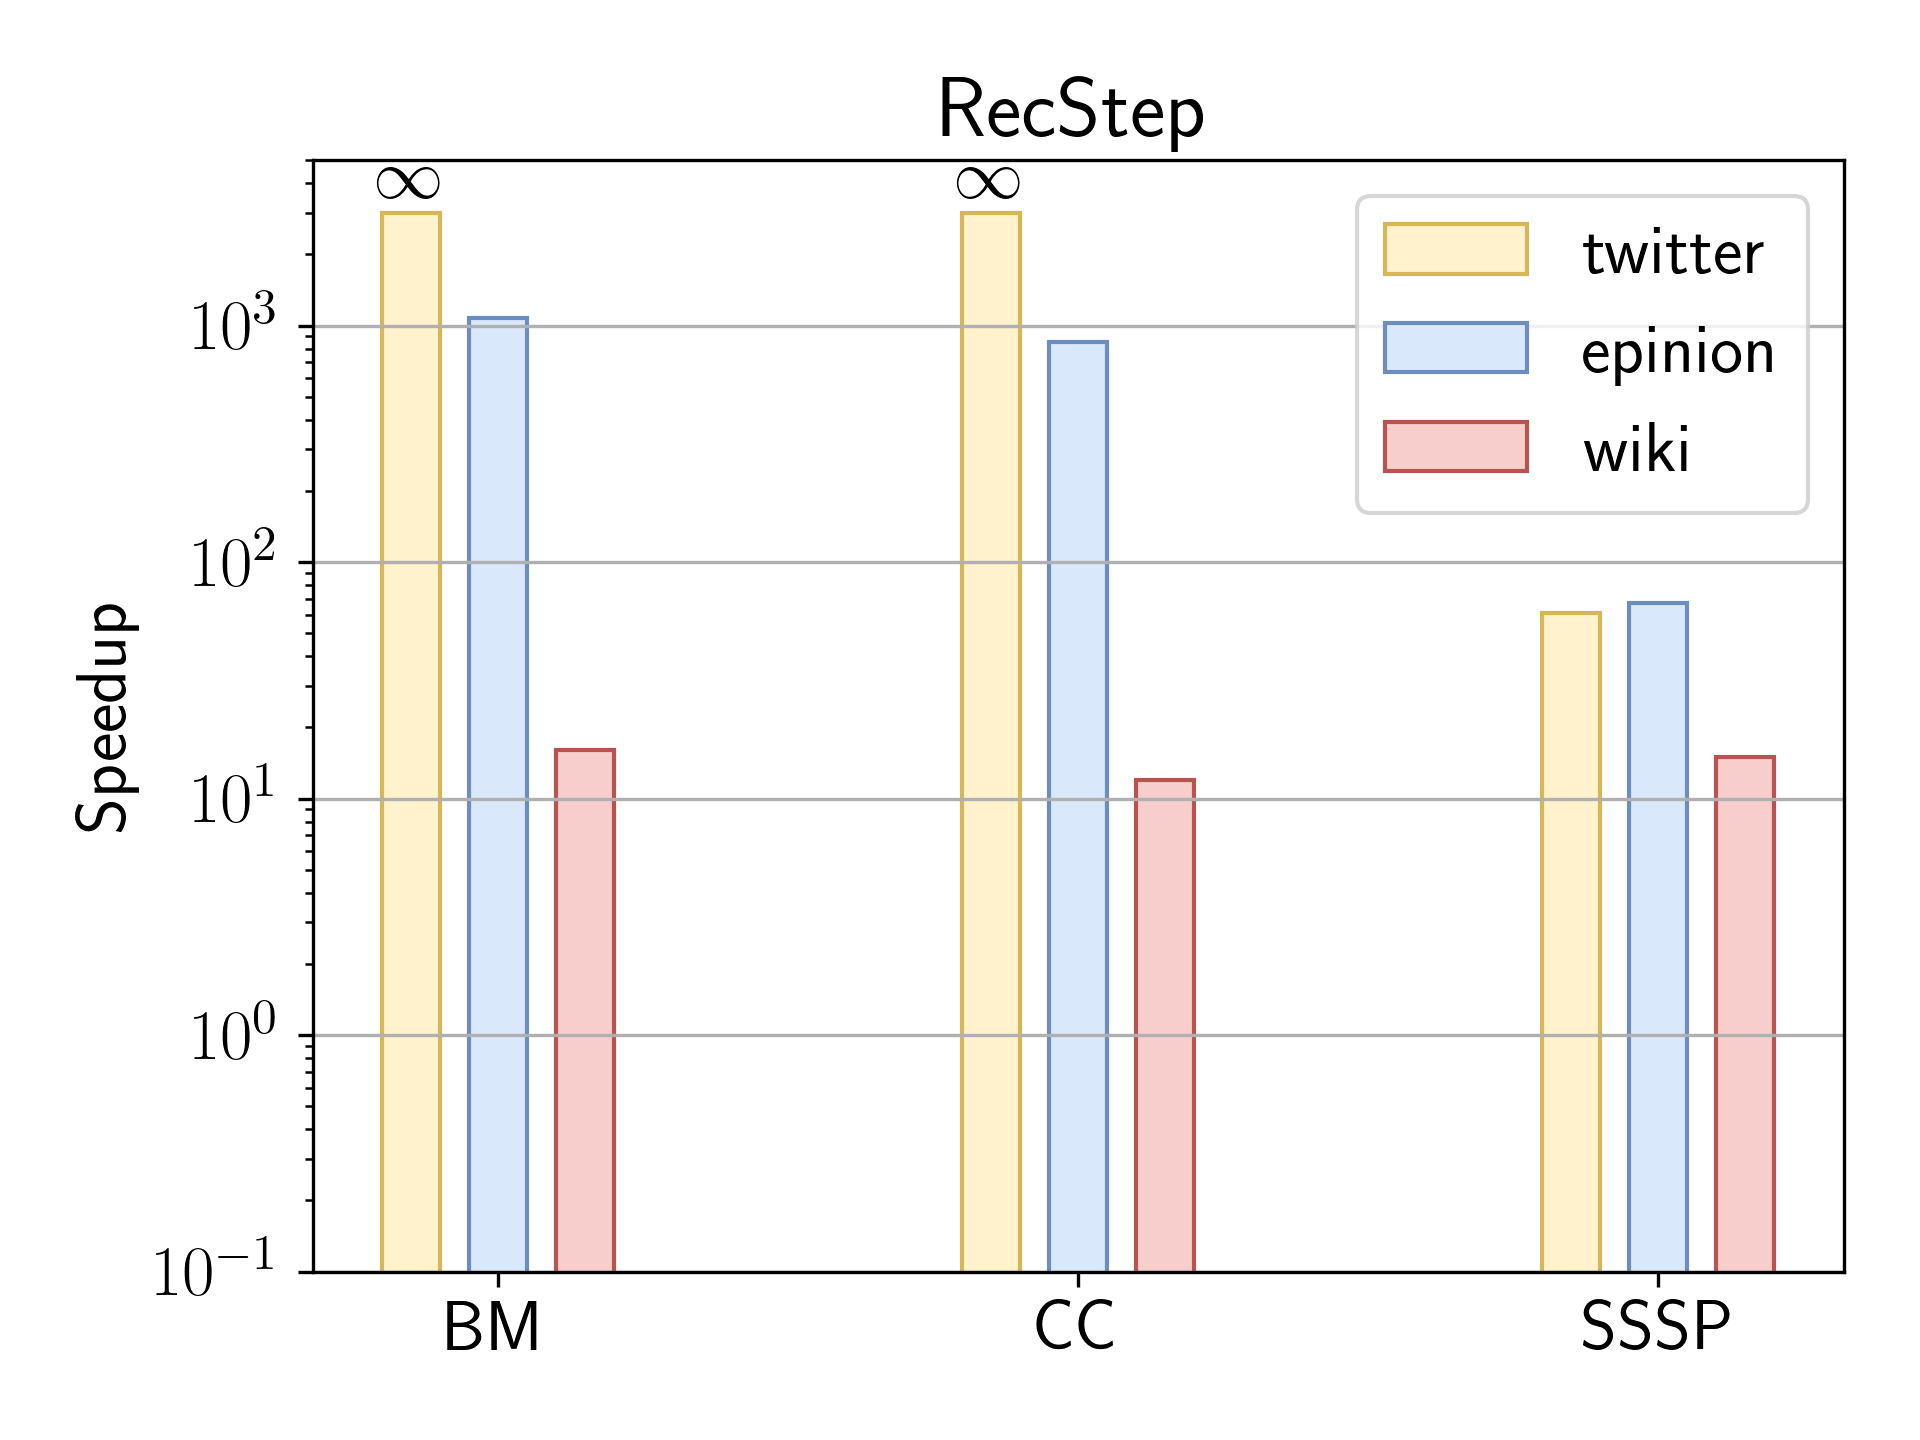
\includegraphics[width=\textwidth]{basic-rs}
        % \caption{RecStep}\label{fig:eval:basic:rs}
      \end{subfigure}

      \begin{subfigure}[b]{0.4\textwidth}
        \centering
        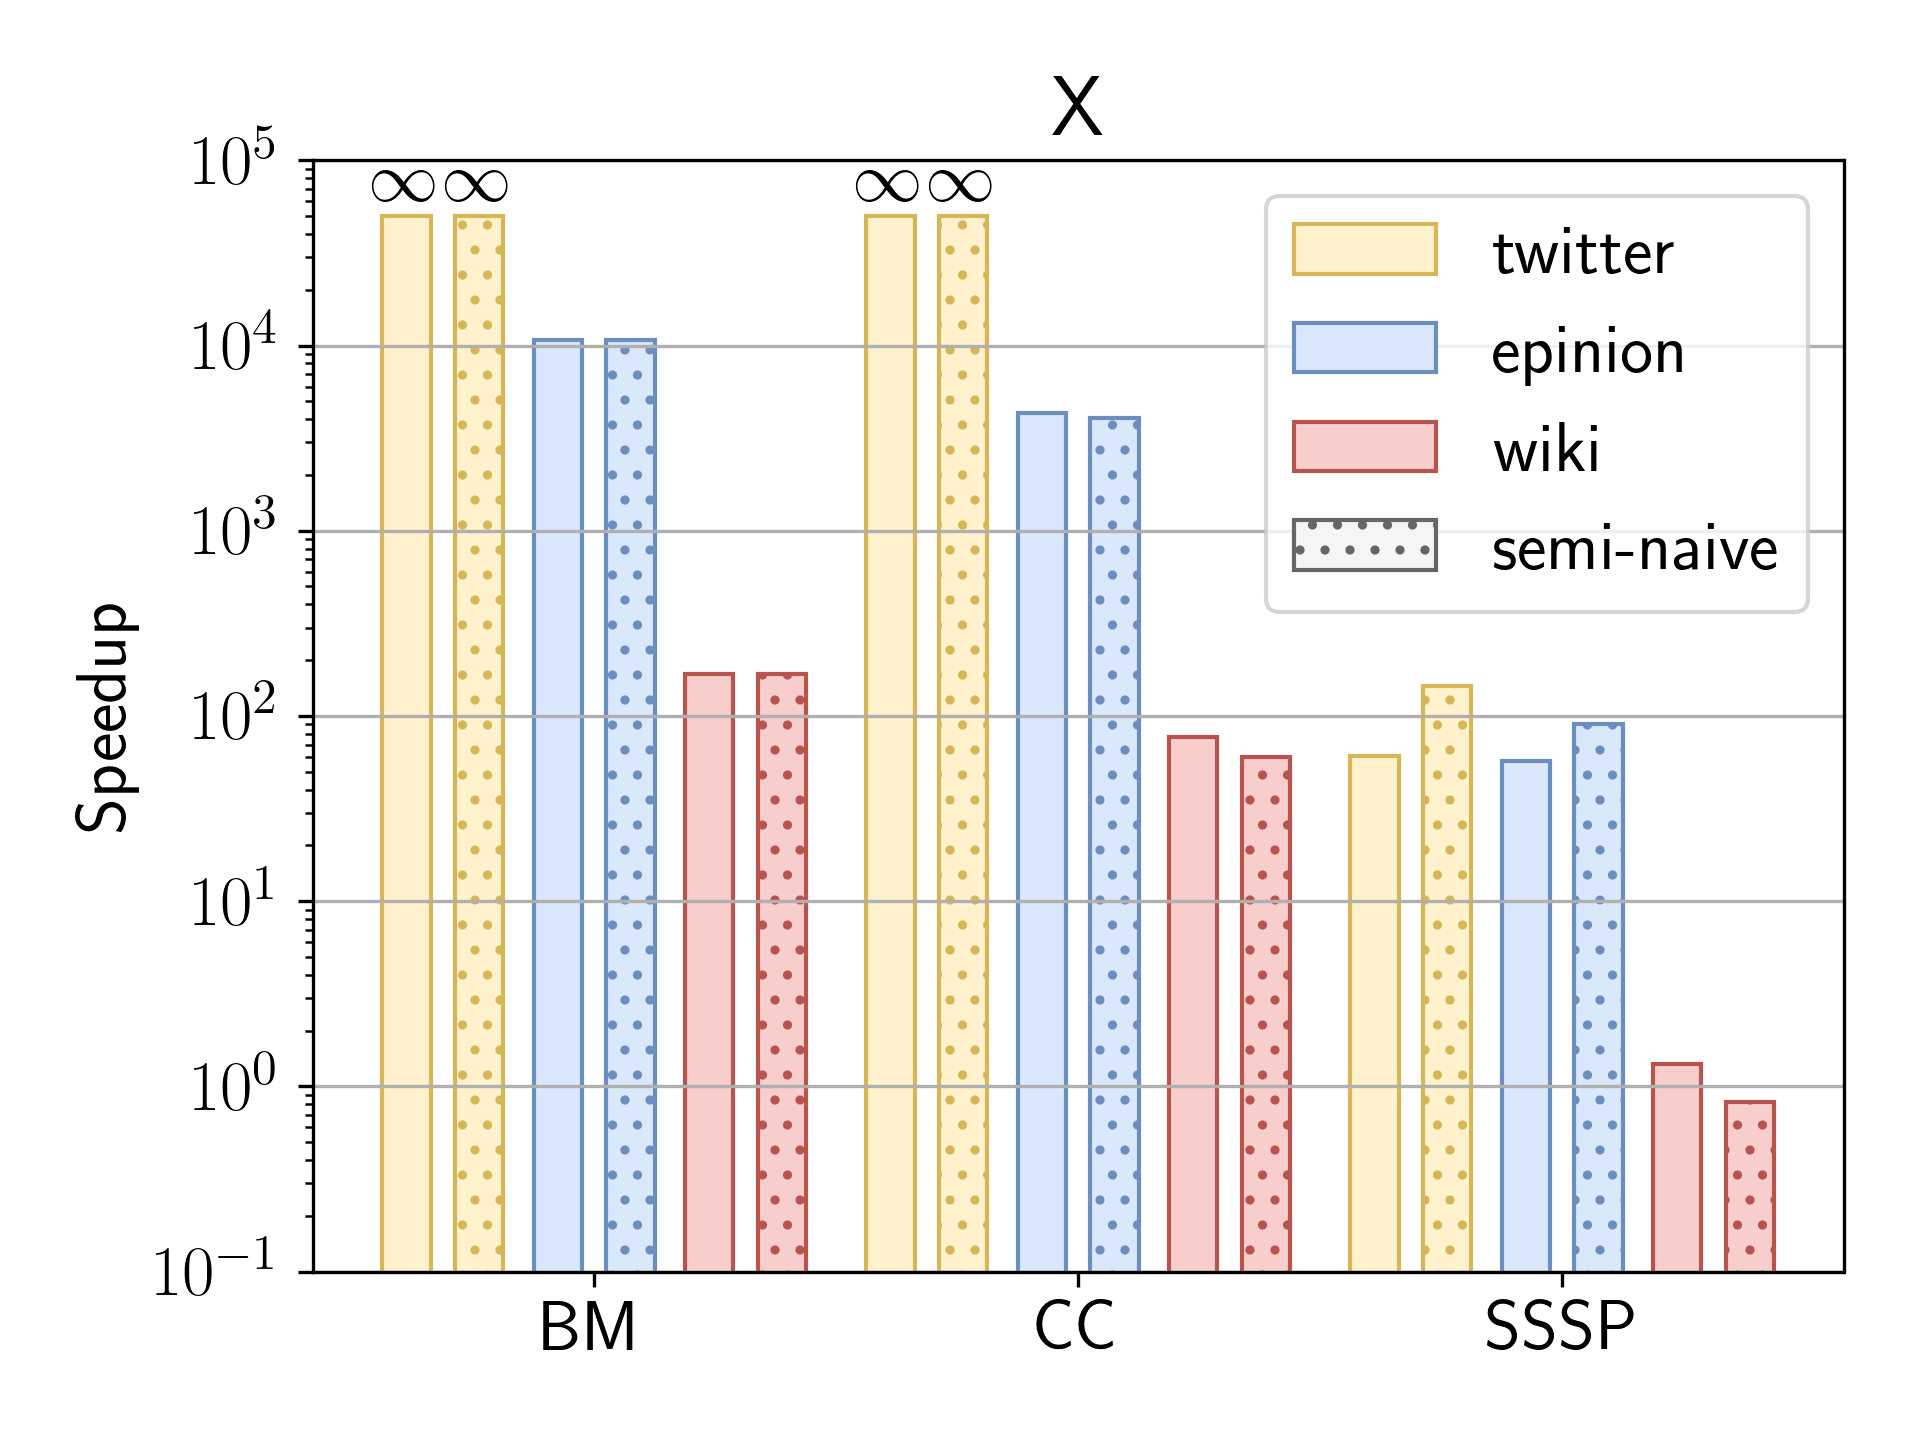
\includegraphics[width=\textwidth]{basic-x}
        % \caption{X}\label{fig:eval:basic:x}
      \end{subfigure}
      \caption*{Speedup of the optimized v.s.\ original program.}
    \end{figure}    
  \end{frame}

  \begin{frame}{Result: Optimizing Recursion}
    SIGMOD'22 (Conditional Accept)
    \begin{figure}
      \centering
      \includegraphics[width=\textwidth]{hard_bench}
      \caption*{Runtime increase as a function of the data size.}
  \end{figure} 
  \end{frame}

  \section{Proposal: Improving Optimizers with Reasoning}

  \begin{frame}{Improving Optimizers with Reasoning}
    A developer of a new system can innovate more freely, 
    but a mature system is difficult to change.

    Relational databases a.la.~SQL are highly mature systems; 
    can they benefit from automated reasoning? 
  \end{frame}

  \begin{frame}{The Cascade Framework}
    Developed for SQLServer~\cite{cascades} and implemented in 
    many SOTA query optimizers. \pause

    Apply a set of \textbf{rewrite rules} to grow a collection 
    of \textbf{equivalent plans}, then extract the best. \pause

    Store plans compactly in a {\em memo table}, where equivalent 
    subplans are grouped into {\em memo groups}.
  \end{frame}

  \begin{frame}{The Cascade Framework}
    Almost identical to equality saturation 
    (e-graph $\mapsto$ {\em memo table}, 
    equivalence class $\mapsto$ {\em memo group}):
    \begin{figure}
      \includegraphics[width=0.3\linewidth]{fgn.pdf}
    \end{figure}
    With one crucial difference: eq.~sat.~maintains 
    \textbf{congruence}.
  \end{frame}

  \begin{frame}{Congruence}
    An equivalence relation $=$ is congruent if:
 \[\forall f : \bigwedge_{i \in [k]} x_i = y_i \implies
  f(x_1, \ldots, x_k) = f(y_1, \ldots, y_k)\] \pause
  \begin{figure}
    \includegraphics[width=0.25\linewidth]{cong1.pdf}
  \end{figure}
  \end{frame}

  \begin{frame}{Congruence}
    An equivalence relation $=$ is congruent if:
 \[\forall f : \bigwedge_{i \in [k]} x_i = y_i \implies
  f(x_1, \ldots, x_k) = f(y_1, \ldots, y_k)\] 
  \begin{figure}
    \includegraphics[width=0.25\linewidth]{cong2.pdf}
  \end{figure}
  \end{frame}

  \begin{frame}{Congruence}
    An equivalence relation $=$ is congruent if:
 \[\forall f : \bigwedge_{i \in [k]} x_i = y_i \implies
  f(x_1, \ldots, x_k) = f(y_1, \ldots, y_k)\] 
  \begin{figure}
    \includegraphics[width=0.25\linewidth]{cong3.pdf}
  \end{figure}
  \end{frame}

  \begin{frame}{Congruence}
    An equivalence relation $=$ is congruent if:
 \[\forall f : \bigwedge_{i \in [k]} x_i = y_i \implies
  f(x_1, \ldots, x_k) = f(y_1, \ldots, y_k)\] 
  \begin{figure}
    \includegraphics[width=0.25\linewidth]{cong4.pdf}
  \end{figure}
  \end{frame}

  \begin{frame}{Congruence}
    An equivalence relation $=$ is congruent if:
 \[\forall f : \bigwedge_{i \in [k]} x_i = y_i \implies
  f(x_1, \ldots, x_k) = f(y_1, \ldots, y_k)\] 
  \begin{figure}
    \includegraphics[width=0.4\linewidth]{cong5.pdf}
  \end{figure}
  \end{frame}

  \begin{frame}{Congruence}
    An equivalence relation $=$ is congruent if:
 \[\forall f : \bigwedge_{i \in [k]} x_i = y_i \implies
  f(x_1, \ldots, x_k) = f(y_1, \ldots, y_k)\] 
  \begin{figure}
    \includegraphics[width=0.4\linewidth]{cong6.pdf}
  \end{figure}
  \end{frame}

  \begin{frame}{Congruence}
    An equivalence relation $=$ is congruent if:
 \[\forall f : \bigwedge_{i \in [k]} x_i = y_i \implies
  f(x_1, \ldots, x_k) = f(y_1, \ldots, y_k)\] 
  \begin{figure}
    \includegraphics[width=0.5\linewidth]{cong7.pdf}
  \end{figure}
  \end{frame}

  \begin{frame}{Congruence}
    An equivalence relation $=$ is congruent if:
 \[\forall f : \bigwedge_{i \in [k]} x_i = y_i \implies
  f(x_1, \ldots, x_k) = f(y_1, \ldots, y_k)\] 
  \begin{figure}
    \includegraphics[width=0.5\linewidth]{cong8.pdf}
  \end{figure}
  \end{frame}

  \begin{frame}{Congruence}
    An equivalence relation $=$ is congruent if:
 \[\forall f : \bigwedge_{i \in [k]} x_i = y_i \implies
  f(x_1, \ldots, x_k) = f(y_1, \ldots, y_k)\] 
  \begin{figure}
    \includegraphics[width=0.5\linewidth]{cong9.pdf}
  \end{figure}
  \end{frame}

  \begin{frame}{Congruence}
    Maintaining congruence is beneficial:
    \begin{itemize}
      \item It can make the data structure more compact 
      \item Which allows exploration to run longer \pause
    \end{itemize}
    Maintaining congruence is non-trivial:
    \begin{itemize}
      \item Naive algorithm runs in quadratic time~\cite{cong} 
      \item Need to efficiently update related data structure
    \end{itemize}
  \end{frame}

  \begin{frame}{Congruence in Cascade-style Optimizers}
    \textbf{Hypothesis}
    An optimizer that maintains congruence can run faster and
    produce more efficient query plans.

    \textbf{Proposal}
    Maintain congruence in Cascade-style optimizers, and investigate
    the impact on the performance of the optimizer \& the 
    plan it produces.
  \end{frame}

  \begin{frame}{Congruence in Cascade-style Optimizers}
    \textbf{Systems to Extend}

    CockroachDB~\cite{cockroachdb} (distributed SQL database):
    \begin{figure}
      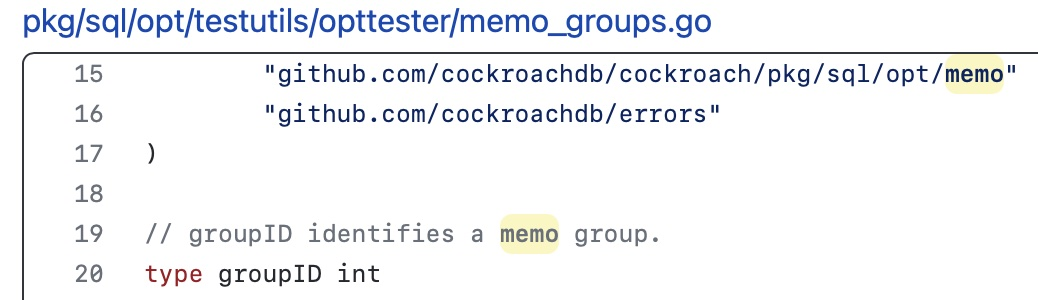
\includegraphics[width=0.6\linewidth]{cockroach.jpeg}
    \end{figure}
    Green Plum Orca~\cite{orca} (Modular optimizer):
    \begin{figure}
      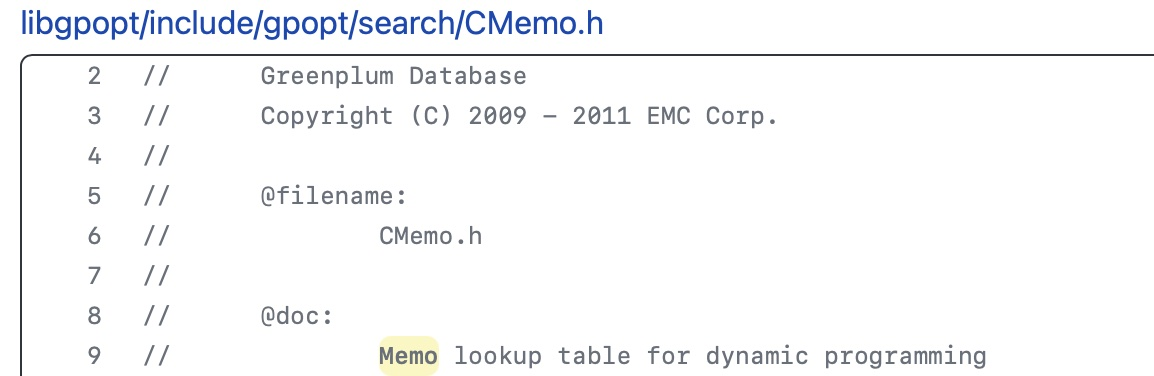
\includegraphics[width=0.6\linewidth]{orca.jpeg}
    \end{figure}
    A SQL verifier by Chu et.al.~\cite{chu}
  \end{frame}

  \begin{frame}{Evaluation}
    Investigate impact on optimizer \& query performance.
    \begin{figure}
    \begin{minipage}{0.3\textwidth}
        \includegraphics[width=\textwidth]{perf.pdf} % first figure itself
        \caption*{Compile time}
    \end{minipage}
    \begin{minipage}{0.3\textwidth}
        \includegraphics[width=\textwidth]{perf.pdf} % second figure itself
        \caption*{Compile memory}
    \end{minipage}
    \begin{minipage}{0.3\textwidth}
      \includegraphics[width=\textwidth]{perf.pdf} % second figure itself
      \caption*{Query time}
    \end{minipage}
    \end{figure}
  \end{frame}

  \begin{frame}{Research Plan}
    \textbf{Hack} Congruence can be implemented as a set of rewrite rules:
    \begin{align*}
      e_1 \bowtie e_2 & \rightarrow e_1 \bowtie e_2 \\
      \sigma_p e & \rightarrow \sigma_p e \\
      \pi_{\mathbf{x}} e & \rightarrow \pi_{\mathbf{x}} e \\
      & \cdots
    \end{align*} \pause
    Suboptimal, but achieves same compression \& query performance \pause
    
    Can serve as a proxy / poor person's congruence
  \end{frame}

  \begin{frame}{Research Plan}
    \begin{enumerate}
      \item Implement congruence as rewrites \& measure performance
      \item If congruence seems ``worth it'', implement an optimal algorithm
      \item Measure performance
    \end{enumerate} \pause
    \begin{figure}
      \includegraphics[width=0.3\linewidth]{poor.pdf}
      \caption*{Performance of congruence algorithms}
    \end{figure}
  \end{frame}

  \section{Conclusion}

  \begin{frame}{Conclusion}
    \begin{itemize}
      \item Core components and techniques from \textbf{automated reasoning}
      can make query optimizers simpler, more efficient,
      and more effective. 
      \item The \textbf{functional representation} of data can enable query 
      optimizers to effectively leverage automated reasoning tools.
    \end{itemize}
    \textbf{Completed projects} \\
    An optimizer for linear algebra based on equality saturation\\
    An optimizer for recursive queries based on program synthesis

    \textbf{Proposal} \\
    Extend a Cascade-style optimizer with congruence.
  \end{frame}

  \begin{frame}[allowframebreaks]
    \frametitle{References}
    \bibliographystyle{amsalpha}
    \bibliography{references.bib}
  \end{frame}

  

\end{document}
